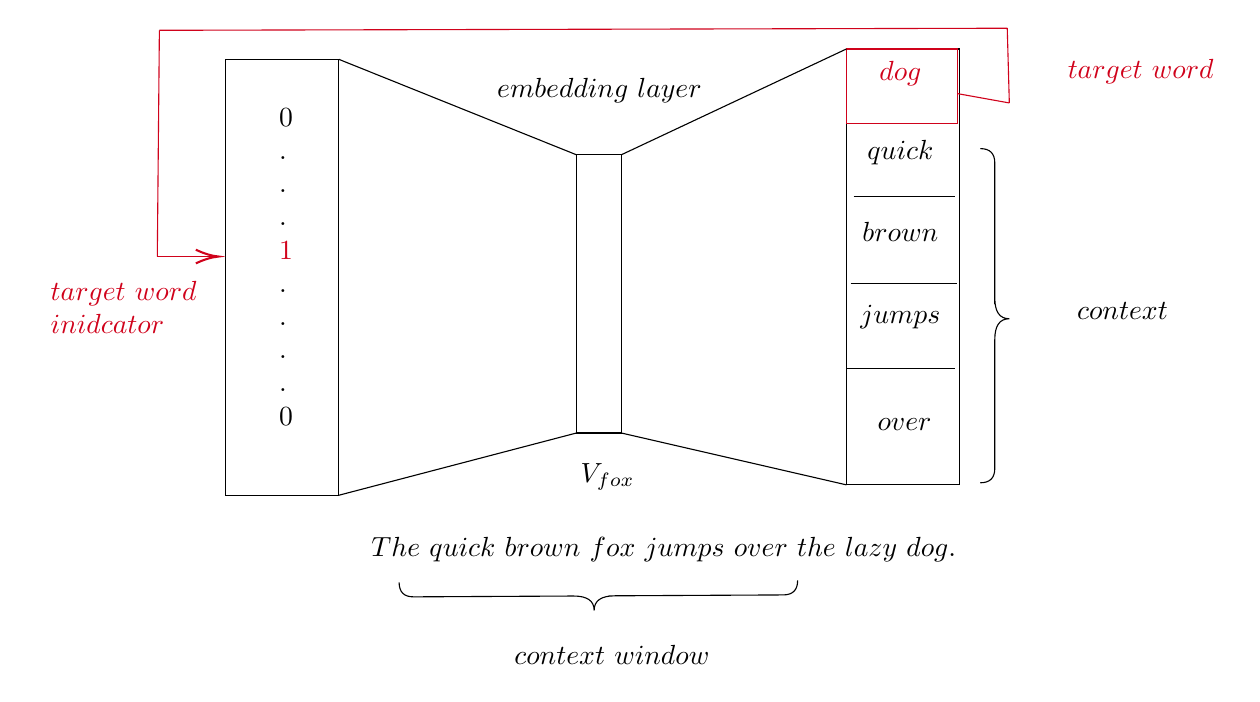
\begin{tikzpicture}[x=0.75pt,y=0.75pt,yscale=-1,xscale=1]
%uncomment if require: \path (0,347); %set diagram left start at 0, and has height of 347

%Shape: Rectangle [id:dp34856826620420023] 
\draw   (288,66) -- (309.5,66) -- (309.5,200) -- (288,200) -- cycle ;
%Shape: Rectangle [id:dp20385411601802828] 
\draw   (418,15) -- (472.5,15) -- (472.5,225) -- (418,225) -- cycle ;
%Shape: Rectangle [id:dp597929679831426] 
\draw  [color={rgb, 255:red, 208; green, 2; blue, 27 }  ,draw opacity=1 ] (418,15) -- (471.5,15) -- (471.5,51) -- (418,51) -- cycle ;
%Straight Lines [id:da329141353304766] 
\draw    (421.5,86) -- (470.5,86) ;


%Shape: Brace [id:dp7412735560954036] 
\draw   (202.5,272) .. controls (202.53,276.67) and (204.87,278.99) .. (209.54,278.96) -- (286.44,278.56) .. controls (293.11,278.53) and (296.45,280.84) .. (296.48,285.51) .. controls (296.45,280.84) and (299.77,278.49) .. (306.44,278.46)(303.44,278.47) -- (387.54,278.03) .. controls (392.21,278) and (394.53,275.66) .. (394.5,270.99) ;
%Straight Lines [id:da1987933863065281] 
\draw    (420,128) -- (471.5,128) ;


%Straight Lines [id:da8961013192322056] 
\draw    (418.5,169) -- (470.5,169) ;


%Shape: Brace [id:dp8413236825652046] 
\draw   (482.5,224) .. controls (487.17,224) and (489.5,221.67) .. (489.5,217) -- (489.5,154.97) .. controls (489.5,148.3) and (491.83,144.97) .. (496.5,144.97) .. controls (491.83,144.97) and (489.5,141.64) .. (489.5,134.97)(489.5,137.97) -- (489.5,70) .. controls (489.5,65.33) and (487.17,63) .. (482.5,63) ;
%Shape: Rectangle [id:dp5223635802427213] 
\draw   (119,20) -- (173.5,20) -- (173.5,230) -- (119,230) -- cycle ;
%Straight Lines [id:da26424324688833556] 
\draw [color={rgb, 255:red, 208; green, 2; blue, 27 }  ,draw opacity=1 ]   (86,115) -- (113.5,115) ;
\draw [shift={(115.5,115)}, rotate = 180] [color={rgb, 255:red, 208; green, 2; blue, 27 }  ,draw opacity=1 ][line width=0.75]    (10.93,-3.29) .. controls (6.95,-1.4) and (3.31,-0.3) .. (0,0) .. controls (3.31,0.3) and (6.95,1.4) .. (10.93,3.29)   ;

%Straight Lines [id:da3427921645180725] 
\draw [color={rgb, 255:red, 208; green, 2; blue, 27 }  ,draw opacity=1 ]   (87,6) -- (86,115) ;


%Straight Lines [id:da5378893688694539] 
\draw [color={rgb, 255:red, 208; green, 2; blue, 27 }  ,draw opacity=1 ]   (87,6) -- (495.5,5) ;


%Straight Lines [id:da1316572119067576] 
\draw [color={rgb, 255:red, 208; green, 2; blue, 27 }  ,draw opacity=1 ]   (495.5,5) -- (496.5,41) ;


%Straight Lines [id:da7079049036395544] 
\draw [color={rgb, 255:red, 208; green, 2; blue, 27 }  ,draw opacity=1 ]   (471.5,36.5) -- (496.5,41) ;


%Straight Lines [id:da6232994776605181] 
\draw    (173.5,20) -- (288,66) ;


%Straight Lines [id:da1671416061216935] 
\draw    (173.5,230) -- (288,200) ;


%Straight Lines [id:da8246799797542117] 
\draw    (309.5,66) -- (418,15) ;


%Straight Lines [id:da7881561473504775] 
\draw    (309.5,200) -- (418,225) ;



% Text Node
\draw (330,256) node   {$The\ quick\ brown\ fox\ jumps\ over\ the\ lazy\ dog.$};
% Text Node
\draw (303,221) node   {$V_{fox}$};
% Text Node
\draw (299,35) node   {$embedding\ layer$};
% Text Node
\draw (562,26) node [color={rgb, 255:red, 208; green, 2; blue, 27 }  ,opacity=1 ]  {$target\ word\ $};
% Text Node
\draw (444,27) node [color={rgb, 255:red, 208; green, 2; blue, 27 }  ,opacity=1 ]  {$dog$};
% Text Node
\draw (444,65) node   {$quick$};
% Text Node
\draw (444,103) node   {$brown$};
% Text Node
\draw (444,144) node   {$jumps$};
% Text Node
\draw (446,196) node   {$over$};
% Text Node
\draw (551,141) node   {$context$};
% Text Node
\draw (305,307) node   {$context\ window$};
% Text Node
\draw (148,121) node   {$ \begin{array}{l}
0\\
.\\
.\\
.\\
\textcolor[rgb]{0.82,0.01,0.11}{1}\\
.\\
.\\
.\\
.\\
0
\end{array}$};
% Text Node
\draw (72,141) node [color={rgb, 255:red, 208; green, 2; blue, 27 }  ,opacity=1 ]  {$ \begin{array}{l}
target\ word\ \\
inidcator
\end{array}$};


\end{tikzpicture}
